
% Introduce the different experiments
% If experiment refer to each other, possibly also mention that here.

\chapter{Results \& Discussion}
The experiments performed during the project have led to many interesting results. Every experiment performed have had great impact on the AIs final performance. Either by presenting the problems and complications that the AI faces during learning or by providing a way to evaluate whether or not the modelling of the environment is sufficient.

This chapter presents and discusses the results that have been achieved during the project. The chapter is divided into sections by experiments performed. Each section presents results as well discussion and reflections about the experiments. The sections also introduce how different experiments and their results relate to each other. The order in which these results are presented follows the order in which conclusions were drawn and the project progressed. Thus one should get a general understanding of the AIs performance improvements during the project from this chapter.

% ----------------------------------------------------------------------------------------
% Refer to the description in method
% Present the results of the experiment
    % - What did it do?
    % - Fitness
    % - Generations required before results
    % - (Population)
% Analyse the results and the meanings behind them.
    % - Was it a good result? Why/Why not?
    % - What conclusions can be drawn from the results?
    % - How could we modify this experiment in order to get additional meaningful results?
% ----------------------------------------------------------------------------------------

% refer to the description in Method
% example: did it help to help in any way
% example: present data
% example: did the hypothesis work
\section{Steering a car moving at a constant speed}
% constant speed -> focus on steering, one variable
% gradually increasing speed, method?
% increasing speed -> push the limits 

%KEY FINDINGS: INTERPRET DATA WELL, FIND COMPLEX BEHAVIOUR, NOT OBSERVED TO OPTIMISE EVERYTHING IN THE SAME SOLUTION(?), HARD TO SEPARATE SIMILAR SCENARIOS, ...

By locking the speed of the car to a constant value, conclusions about the AIs ability to steer the car could be drawn. The constant speed was gradually increased with the goal to force the AI to drive more intelligently and to find its limitations. 

Noteworthy is that after the car completes a track, rewarding it for improved time or improved distance driven is analogous. Since the car is driving at a constant speed, this will only result in a shorter distance being driven to get around the track.

The experiment was performed in two ways, one where the AI can look further down the track and one where it only has local knowledge about the track. Results for each of these sub-experiments are presented in the subsections below.

\subsection{Only local perception}
Providing the system only with local perception and giving it control of the steering, as explained in section \ref{method:constant_speed}, present successful and interesting results. The system immediately learns that positioning the car in the middle of the track at all times is preferable. Given that the system only has knowledge about the local relation between the car and the track, this behaviour is reasonable.

On straights this behaviour works well, it could even be considered optimal behaviour in some scenarios, however in corners it is not. When the car approaches a corner the middle of the track is shifted, causing the car to become out of position. At this point, the system tries to adjust the cars position. Before the system has had sufficient training, the amount of steering performed is either to large or too small. To large of an adjustment causes the car to oscillate between the middle line of the track, which eventually causes the car to crash. To small of an adjustment instead results in the car not getting back to the middle, eventually causing the car to crash as well. It has been observed that the oscillation occasionally helps the car to complete a complicated corner, by positioning the car in a good way. Even though this behaviour improves fitness and in theory could make the car complete the lap with a higher constant speed, the behaviour is not target behaviour. Oscillating between the middle of the track is not an optimal behaviour in racing.


%Text prior table
% The amount of training required to take a complete lap, if possible, is dependent on the constant speed of the car. At a constant speed of 10 m/s it takes two generations for the car to take a complete lap. At this point the oscillation has stopped, and the car follows the middle of the track at all times. Increasing the constant speed to 11.6 m/s, causes the generations required to perform a complete lap to increases to five generations. At 11.7 m/s the generations required were 22. At these speeds, the car switches between oscillating and doing too small of a steering adjustment, causing the car to crash. When the car eventually completes a lap, there is no oscillating behaviour. Further increasing the speed, caused the car never to complete the lap. This also caused the oscillating never to stop, due to the turning radius being too small to complete a corner when sticking to the middle of the track.

The amount of training required to take a complete lap, if possible, is dependent on the constant speed of the car as seen in table \ref{tab:localdata}. Before a the lap were completed, the car would oscillate over the track. However, at these speeds, the oscillating behaviour would disappear. For speeds higher than $11.7$ m/s, caused the car never to complete the lap. This also caused the oscillating to never stop, due to the turning radius being too big to complete a corner when sticking to the middle of the track.

\begin{table}[h!] 
  \centering
  \begin{tabular}{ll}
    \toprule
    Speed [m/s] & Generations\\
    \midrule
    $10.0$ & $2$ \\
    $10.6$ & $5$ \\
    $10.7$ & $22$ \\
    \bottomrule
  \end{tabular}
  \caption{Data of how many generations required until a genome with a constant speed could take a complete lap with local perception}
  \label{tab:localdata}
\end{table}

This experiment can in general be considered a success. It was confirmed that NEAT can find behaviours that are applicable to steering a race car, and in some scenarios it can even find optimal behaviours. It is however impossible for this solution to sophistically prepare for an approaching curve. The only way for the system to determine whether or not the car should turn, is based on the current distance from the middle of the track. Which does not tell it anything about the corner in front of the car. It would be interesting to see how the system reacts to information about the upcoming part of the track. Is it possible for the system to plan ahead, in order to position the car such that it can travel through tough corners with higher speed?

\subsection{Local perception and track curvature}
\label{subsec:fixedspeedcurvature}

When using the track curvature data in addition to the local perception, solutions that completed the track was found up to 12.1 m/s. It is 0.4 m/s more than was found not using the curvature data. The difference in speed may seem small, but the difference in behaviour is substantial.

What the solutions found generally do is that they position themselves well before a curve, to compensate for the larger turning radius required. They also start to steer before the curve actually start.

\begin{figure}[h]
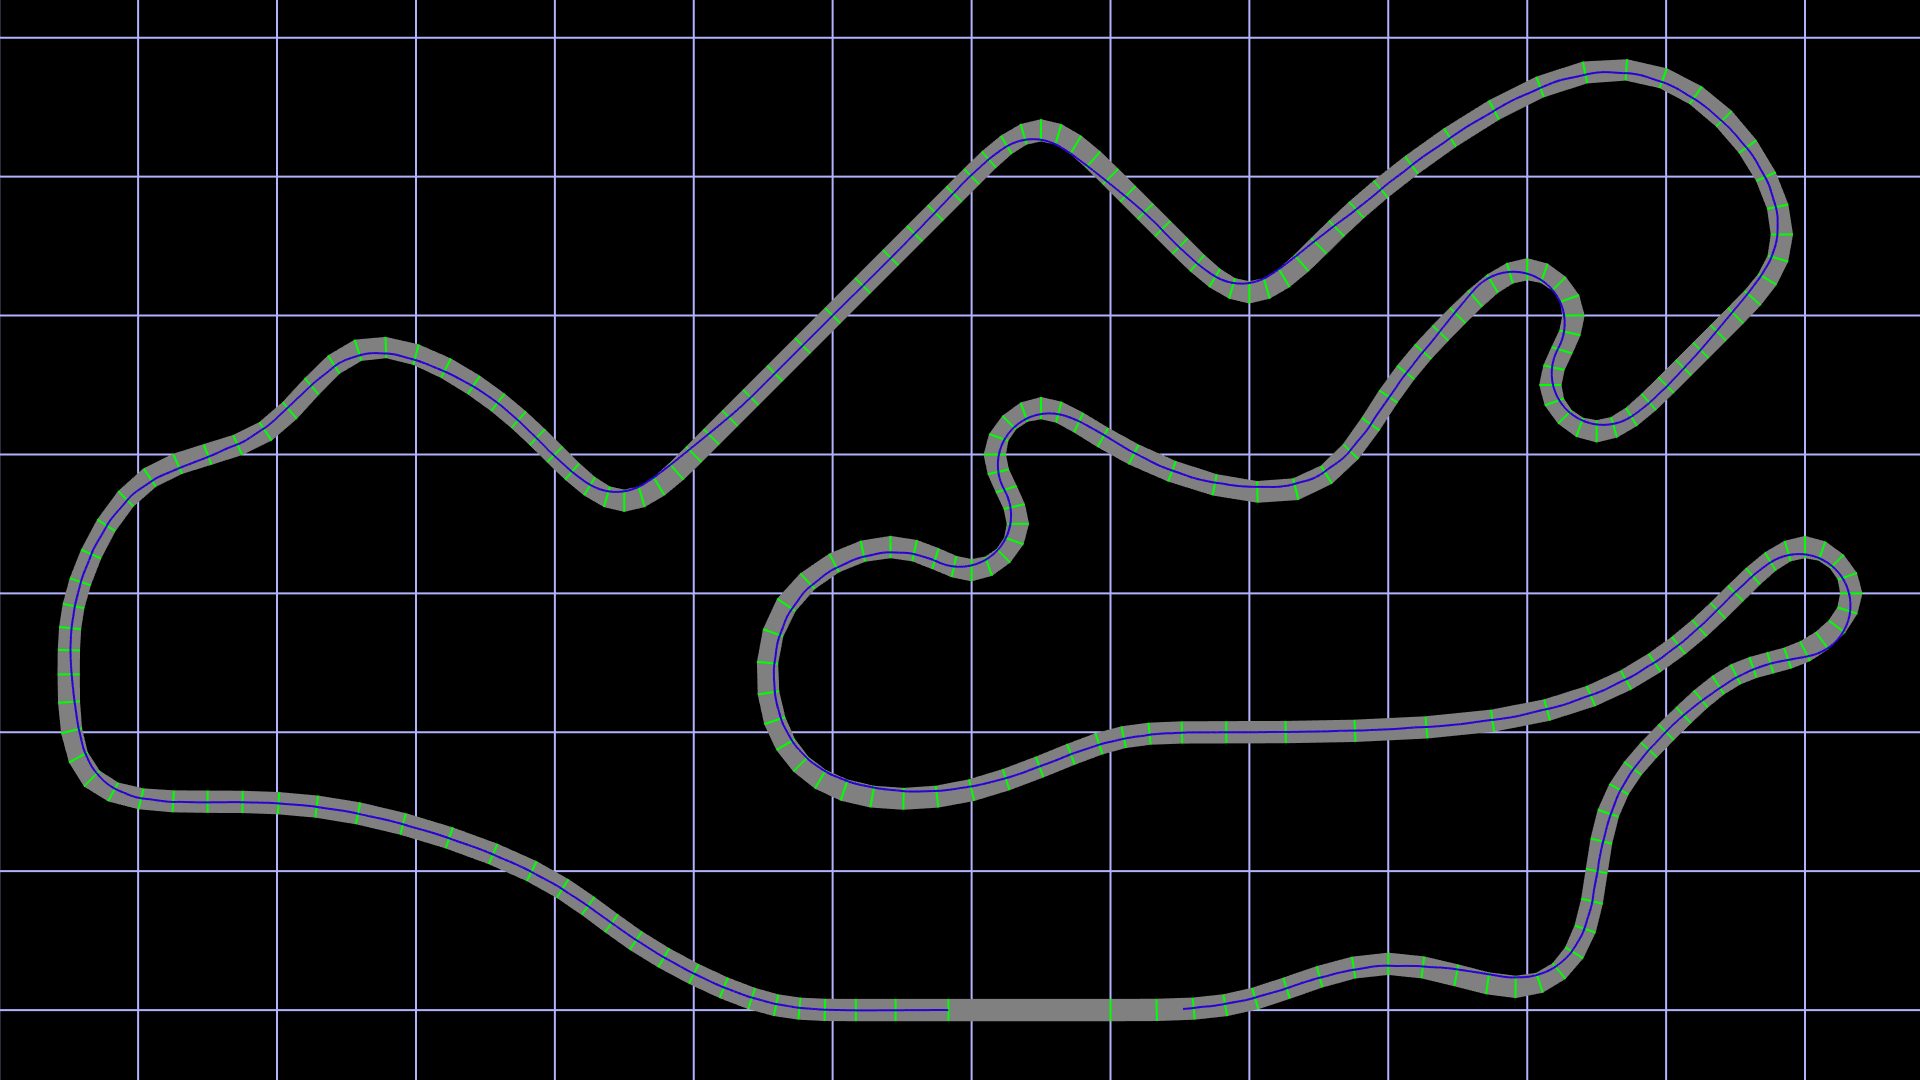
\includegraphics[width=\textwidth]{report/images/fixed_curve_data}
\centering
\caption{Showing a clockwise race line from the best found genome with a constant speed of 12.0 m/s.}
\label{fig:constantspeedline}
\end{figure}

The speed that provided the most correctly looking race lines was 12.0 m/s, whose race line can be seen in figure \ref{fig:constantspeedline}. At that speed the AI had to push the limits in order to manage the sections with the most corners as seen in figure \ref{fig:constantspeedsection}. This experiment completed the whole track in $356$ generations, and the fastest time to complete the track in was $415$ seconds and was reached after $1225$ generations. The race line created by this experiment is almost as good as it can be at this constant speed. 

\begin{figure}[h]
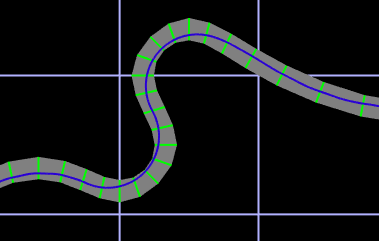
\includegraphics[width=\textwidth]{report/images/constant_speed_section}
\centering
\caption{Showing the race line in a section from the best found genome with a constant speed of 12.0 m/s. The sections is driven from right to left in this section.}
\label{fig:constantspeedsection}
\end{figure}

When the speed increased, the AI had to start turning very late in the section displayed in figure  \ref{fig:constantspeedsection}, to make a little more space for the following curve. This made it less interesting to investigate further, since that behaviour resembled real behaviour less.



% Check for longer training sessions
Each of the solutions found showed some typical characteristics. If one solution managed to drive tightly to the inner side in the toughest curve or positioned itself extremely before a curve, it also showed that tendency for all other mayor curves. On the contrary, if it turned late in the tough curves, it also did it for the other curves too.

%Check for longer training sessions
The recurrent characteristics in the behaviour for a particular solution often had one limitation, that they failed to manage simpler as efficient as the tough curves. If the solution managed to take the tough curve, near optimally, we never observed that it also managed to take the simpler curves as efficiently. For example, for the lightly turning curves, the car always drove a few meters from the edge of the track, even if it certainly had traction to stay closer. 

%Check for longer training sessions
It seemed like it did not learn to distinguish properly between the different difficulties, and simple did the same behaviour in miniature. Worth noting was that these training sessions lasted for only about 2-600 generations. We have not proven that it is not possible if one trains for longer.

%OLD: The best network found for the speed 12.0 (SPEED 50????!!!?!??!!) had fitness 5821.93. It had a total of 9 hidden nodes, a total of 20 edges, 8 edges within the hidden layer, 4 to output nodes, 9 of the input nodes and bias was connected (0, 1, 3, 4, 5, 7, 8, 10, 13, 15) (bias, distance to middle, distance to right edge, angle to mid line, curve data points 10m 42m 66m 144m 397m and the segment sum of the first four points in the region 10-66m) (Remember to check which edges are enabled!)


\subsection{Shortest path}

The fastest route for a car that moves forward with a constant speed is the shortest one. This means that the only way for a genome to increase its fitness once it completes the circuit is to decrease the distance driven around the track.  

The result show that after the algorithm finds specimens that are able to complete the circuit, the gene pool continues to improve. The path around the circuit is shortened to a great extent. The difference in length of the race line and the middle line of the circuit is significant. 

The optimal behaviour is intuitively to always drive on the inner curves and to drive a straight line between the curves where it has to turn. Small variations on the curvature should not matter, if the edge does not intersect with the path the car drives.

The car follows the key behaviour aspects, but not to the extent that the path is optimal. We can see that it drives tightly to the inner side for very tight curves, but not for low intensity curves.

%Training times...

%Network structure...

% NOTE: Data based on speed_and_control_run_1
\section{Full control of the car}
% Beteendeanalys
% - It does not brake/accelerate before/after curves. Why is this? Could the input potentially be modified, such that it is easier for the system to realise what needs to be done? Distance to next curve? 

% Analysis
%X - Can it manage to learn many components of the behaviour at the same time? Adding one more component only may make the performance worse


The base experiment performed, as explained in section \ref{method:baseline}, gives the possibility of controlling the cars throttle. Adding the concept of controlling the throttle has led to an increase in complexity that was more significant than was anticipated. By looking at the results from training sessions, one can see that the complexity of the computations increases significantly.

It takes 98 generations until the training process reaches a point where one genome can perform a complete lap. The behaviour observed after 98 generations is one that drives at a constant, slow pace along the track. The car travels $5200$ meters in $1110$ seconds. Between the corners, the car travels in a straight line parallel to the track. The position at which this line is relative to the tracks mid line changes when the car goes through a corner.

After a genome manages to complete a lap, the data shows that the training process actually manages to find genomes that can drive faster and faster around the track. The process of finding a genome that reaches all the way around is less time consuming than the process optimising for time. As seen in figure \ref{fig:steerspeeddata} on page \pageref{fig:steerspeeddata}, the best genome of each generation increases rapidly until the fitness exceeds fitness of 5200. As this level of fitness have been reached, the training process have a gradual curve compared to the steep curve before reaching fitness of 5200.

\begin{figure}[h]
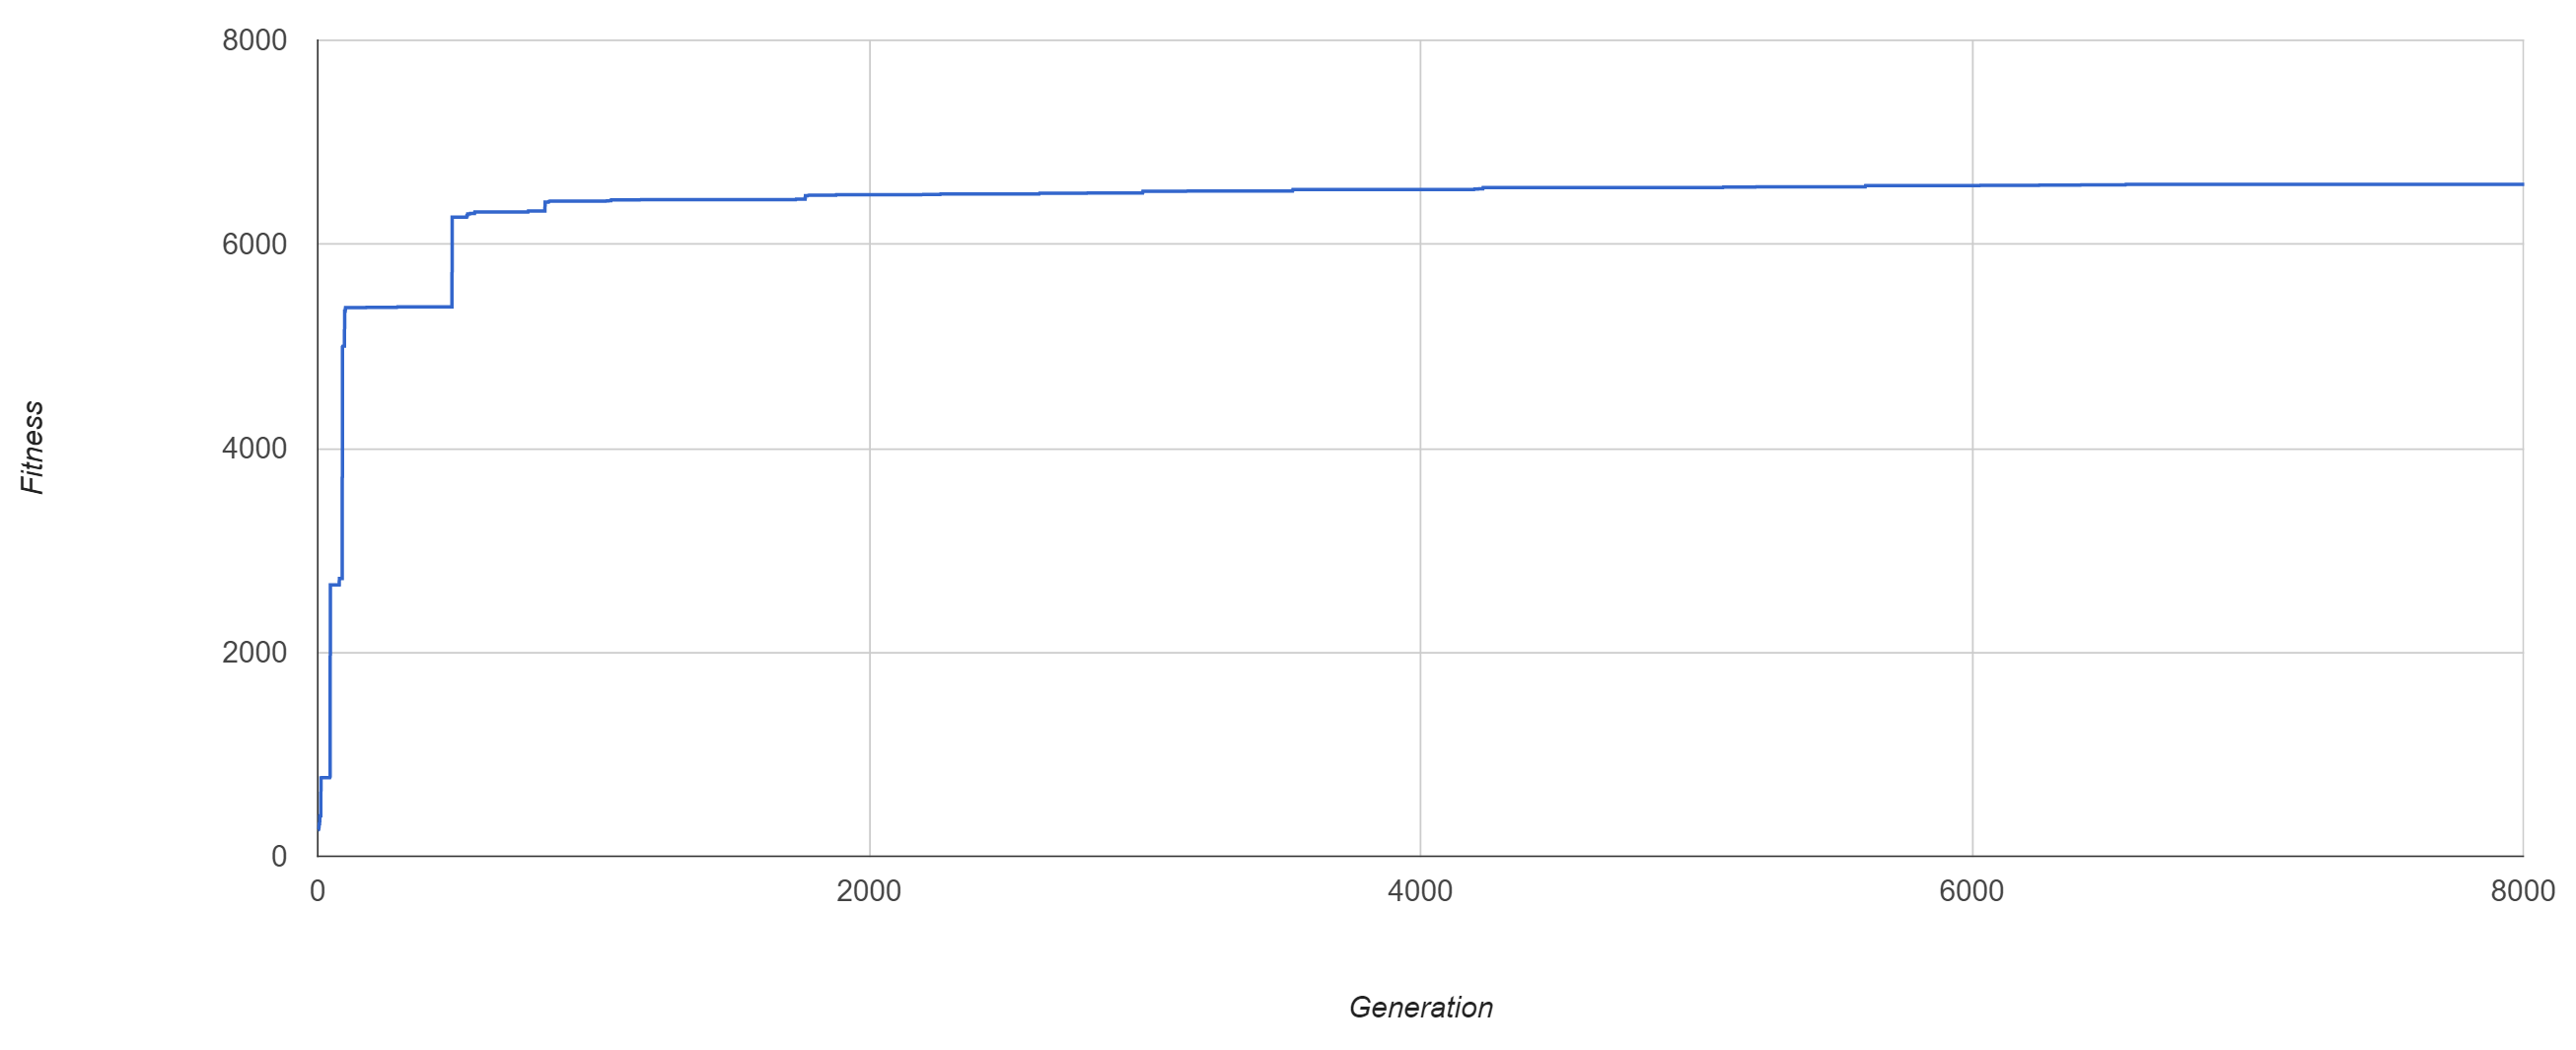
\includegraphics[width=\textwidth]{report/images/graphs/steeringandspeedcontrolrun1}
\centering
\caption{Showing best fitness of each generation. Note that after 98 generations the fitness value surpasses 5200 as the circuit have been completed.}
\label{fig:steerspeeddata}
\end{figure}

A fitness of $6587.56$ was the highest value that was reached during this experiment. Reaching this fitness value took $8331$ generations, and it corresponds to completing the track in $490.68$ seconds. Even though the system manages to lower the lap time quite significantly, the final result is not optimal. As seen in figure \ref{fig:steerspeedline}, the path taken by the car still resembles the one that was found at generation 98.

\begin{figure}[h]
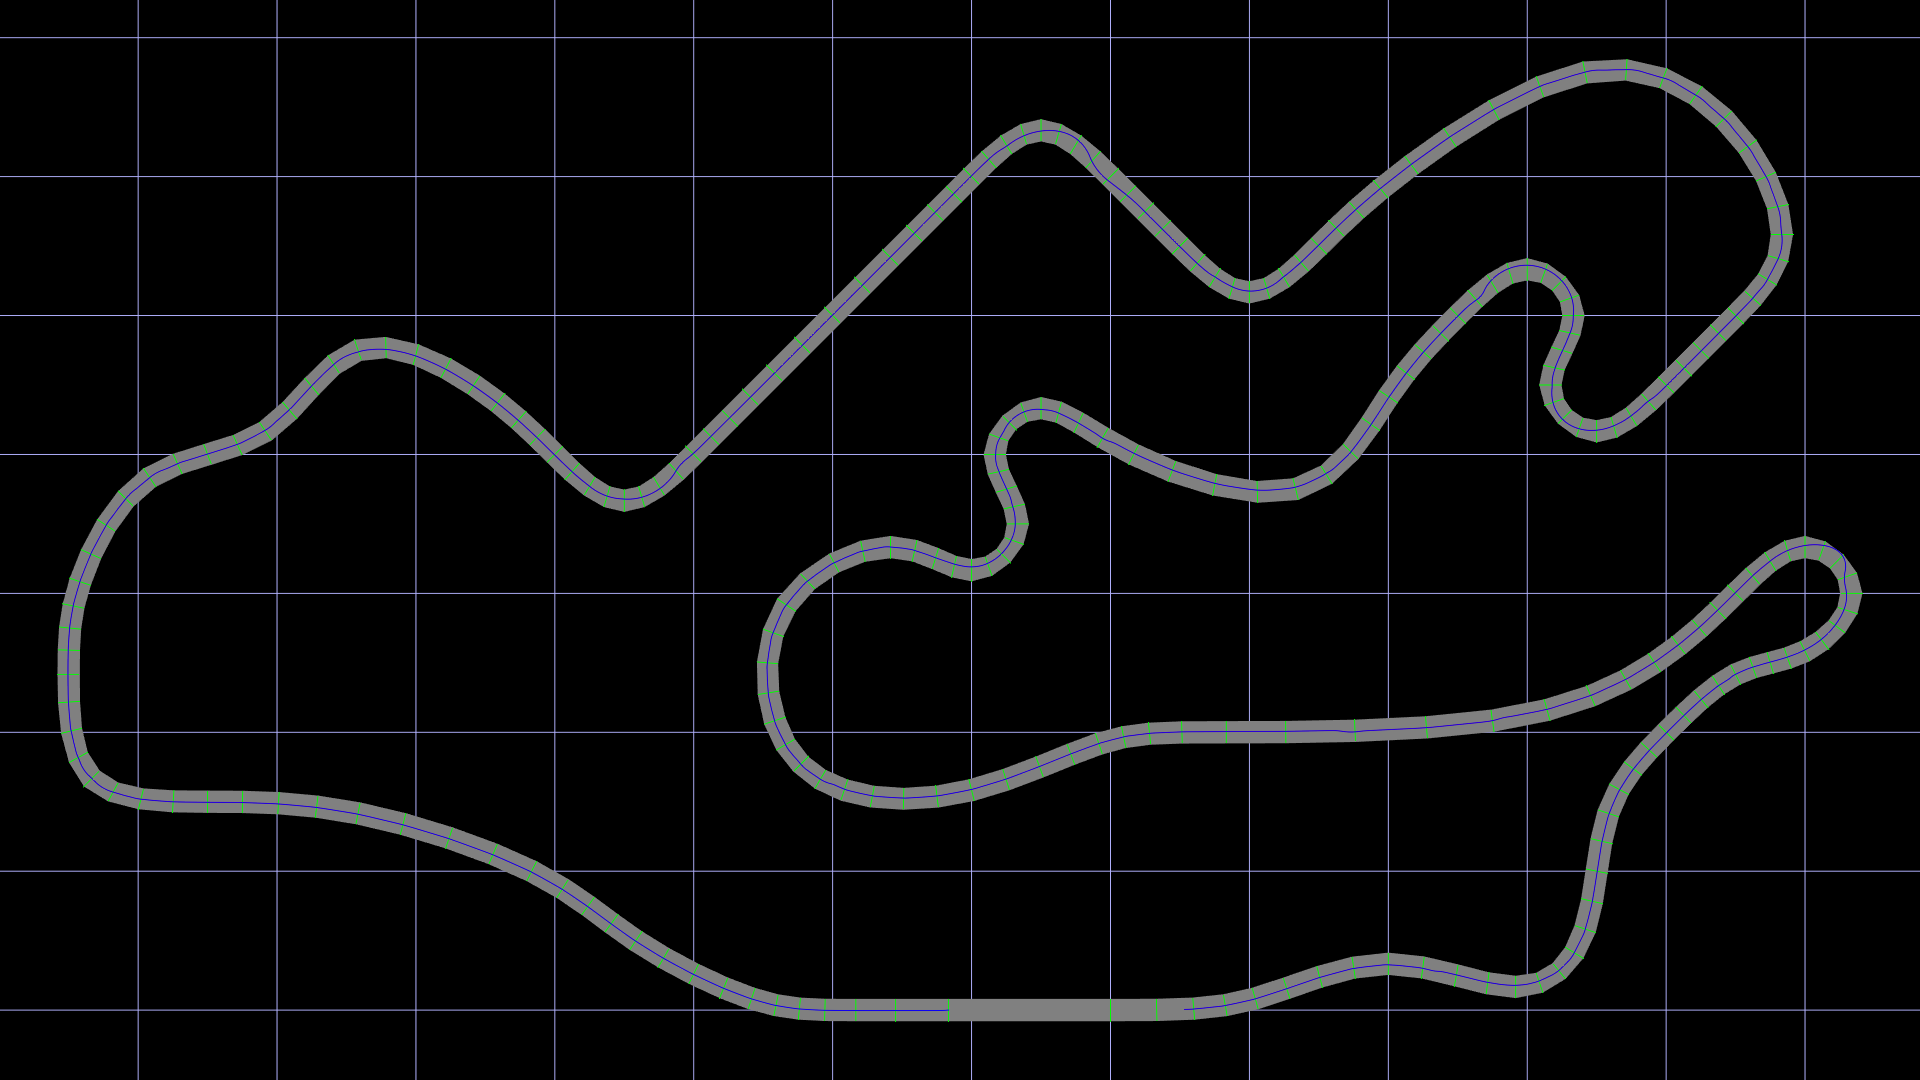
\includegraphics[width=\textwidth]{report/images/normal_generation_6558}
\centering
\caption{Showing a clockwise race line completed by a genome with a fitness value of 6587.56, the best fitness reached in the steer and speed control experiment. The speed of the car is presented by the line colour, with blue as slowest possible speed and red as max speed.}
\label{fig:steerspeedline}
\end{figure}

% - It does not brake/accelerate before/after curves. Why is this? Could the input potentially be modified, such that it is easier for the system to realise what needs to be done? Distance to next curve? 
The increase in lap time has been observed to be based on two improvements. The first one being the fact that the average speed around the track has increased significantly and the second one being the increase in acceleration and breaking during turns. It has been observed that the car accelerates during the straights and brakes before corners, although very small amounts of acceleration and braking. In order for this behaviour to properly increase the performance of the network, it would have to be more extreme.

% The lines that were taken by the best genome can be seen in figure \ref{fig:steerspeedline}. This figure shows that the car does not hold a constant speed throughout the complete track. It can be seen that the car accelerates the slightest at the straights, to use the brake as an action not to hit the wall. This behaviour would need to be more extreme to minimise the time to complete the track; at the current extent, the behaviour is not enough to become faster than the best constant speed genome.

% - How do the behaviour / performance differ to the fixed speed.
    % - The amount of training required is a lot higher. Compared to ~1000 generations of fixed speed, which resulted in an almost perfect race line.
    % - Its similar to fixed speed, but a little bit worse.
    % - Its similar to fixed speed in time during the laps, fixed speed with 12.f is a little bit faster. (Include details)
    % - When it comes to race lines, fixed speed is A LOT better. Introducing the steering/breaking output makes the performance worse in general. Why?
% Even though this genome has the ability to control the break and throttle, it holds a lower average speed than the best genome that performs a complete lap in the constant speed with curvature experiment.
% Compared to the results in section \ref{subsec:fixedspeedcurvature}, the fastest genome in this experiment time is slower than the best genome in the corresponding constant speed experiment. 
Even though the system has the ability to control the break and throttle in this experiment, it performs worse than the best genome in the constant speed with curvature experiment. By a $1000$ generations the constant speed with curvature experiment presents an almost optimal race line for the constant speed. While the best genome in this experiment performs a lap, it does so by simply driving along the track mid line. Although the race lines are significantly different, the lap times are not. Compared to $415$ seconds in constant speed with curvature, this experiment performs a lap by $533$ seconds.

Since the system is capable of finding almost optimal race lines, as seen in the constant speed with curve data experiment. It is clear that when the system is given the ability to accelerate and brake, the performance is altered. The increase in outputs and possible actions, creates a much more complex environment that requires more computation to achieve the same level of results as a system that utilises constant speed. This results in worse performance overall.

It is interesting to consider that the system seems to get stuck in specific paths. Since the path cannot be modified, the race line will not allow for an increase in speed through the corner. It is possible that the network becomes over trained on a specific behaviour before it is allowed to optimise for time. Thus it might be beneficial to research the possibility of optimising for time before performing a complete lap. 

% Another important aspect/behaviour is that the car is almost in the middle of the track all the time. The line taken by the car only diverges from the middle in the most difficult corners. The constant speed experiment has given a more active line that can be seen at figure \ref{fig:constantspeedline}. The fixed speed line is taking the corners much better, and it can also position the car prior a corner to make a better turn. This is a behaviour that this experiment is missing.

% When the system is given the ability to accelerate and decelerate, it is clear that the performance is altered. The increase in outputs and possible actions, creates a much more complex environment that requires more computation to achieve the same level of results as a system that utilises constant speed. This results in worse performance overall.

\section{Short track segment}
\label{result:short}
As hypothesised in section \ref{subsec:shorttracksegment}, the system is able to find more effective behaviours on shorter tracks than on the complete circuit. The behaviours found of the three track segments are not perfect, however they show signs of effective speed management, which is one of the criteria looked for the in the behaviour. The genomes do not show any significant signs of effective positioning, which is the other major criteria. 

In each experiment the most successful genomes keep a high speed until braking before the corner and accelerate out of the corner, keeping a high speed until the end of the track. 

\begin{figure}[H]
    \centering
    \subfloat[Race line going through 30-degree corner.]{{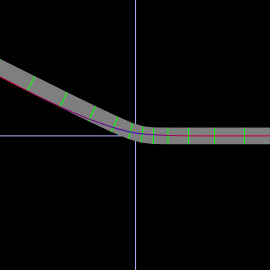
\includegraphics[width=0.28\textwidth]{corner_30_result}}}%
    \qquad
    \subfloat[Race line going through 90-degree corner.]{{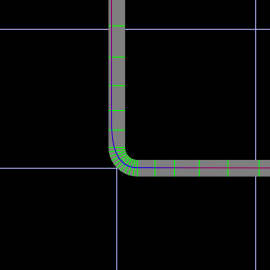
\includegraphics[width=0.28\textwidth]{corner_90_result}}}%
    \qquad
    \subfloat[Race line going through 180-degree corner.]{{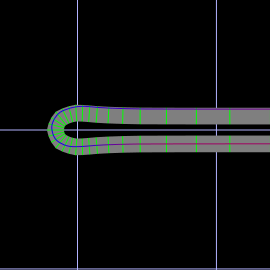
\includegraphics[width=0.28\textwidth]{corner_180_result}}}%

    \caption{Aerial view of the race lines through the three corner types. The grey line is the track which is 12 metres wide. The race line goes from red, to blue and back to red. The colour represents the speed of the car, were red is fast and blue is slow.}
\end{figure}

Even though the system did not find any near perfect behaviours, the results show that the system has a greater ability to optimise for time when training on shorter tracks. One plausible reason behind this is as mentioned in section \ref{subsec:shorttracksegment} that it is too hard to change the behaviour of the genomes are able to complete the circuit. In order change from a cautious behaviour to a more effective one the genome must learn to accelerate on straights and brake before corners at the same time. Changing only one aspect at a time will most likely lead to a worse behaviour. If a genome is changed to accelerating more it will likely crash in a sharp corner. Likewise, if a genome is changed to braking before corners without accelerating more it will drive slower and thus decrease in fitness.  

%\section{Multiple short track segments}
% Ta tillbaka till slutinlämning 

%%% KÖTTA UT


\section{Mirrored track}
% TODO: Sätt in grafer och skit.
\label{result:mirror}
The experiment where the training environment was exchanged to a mirrored version of the same track showed several interesting results. The test population was trained on the normal circuit until the best specimens managed to complete the circuit in approximately $500$ seconds, which took $3527$ generations with a population of $500$ genomes. That population was then transferred to training on the mirrored track. On the first try, some specimens managed to complete $1800$ metres of the circuit which is about a third of the way. This shows that at least some of the genomes had some general knowledge about how to drive. However, in the next few generations the population managed to complete the whole circuit. This is much faster than the control population which took approximately $150$ generations to complete the circuit. 


\begin{figure}[H]
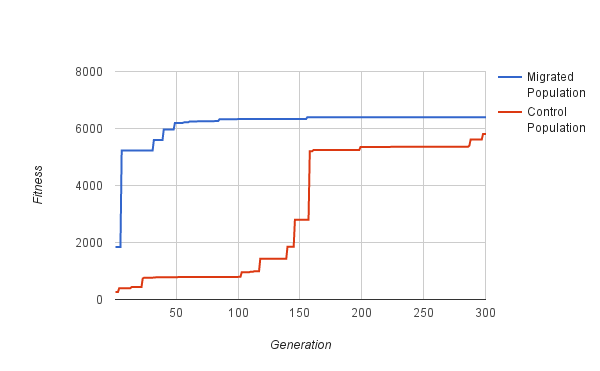
\includegraphics[width=\textwidth]{report/images/graphs/mirror_migration}
\centering
\caption{Showing the fitness progression of the migrated population shown in blue and the control population shown in red. Note that the migrated population in a few generations surpasses a fitness-value of 5000 as a result of completing the circuit.}
\label{fig:mirrordata}
\end{figure}

This shows that some of the knowledge acquired on the first track is applicable on the second. The reason may be that the genomes are adapted to similar corners on the first circuit or that the algorithm has found a driving function based on the provided inputs that is applicable in a wide range of situations. In either case, one could argue that in order to find a generalised behaviour the AI should train in an environment where it encounters a wide range of situations, which in the racing domain would be different corners or combinations of consecutive corners. 

% Skriv om bajsiga meningar.
The extension to the experiment where the migrated population was migrated back to the original circuit once it had adapted also showed interesting results. The population forgets knowledge when adapting to the new environment. This is somewhat expected since the population mutated for 500 generations on the mirrored track, ergo no genomes trained on the original circuit remain in the population. However not all of the knowledge is lost in the process, some generalised knowledge remains. When migrated back to the original track, one specimen manages to stay on the track for circa $2800$ metres, which is slightly past halfway around. After only $5$ generations of adapting back to the original track one specimen manages to complete the circuit, albeit slowly. The adaption to the original circuit is similar in nature to the adaption from the original to the mirrored one. 

These results show that the system is able to find generalised knowledge to some extent. However, the results also show that some knowledge acquired on the original circuit is lost during the training on the mirrored one. This is possibly due to the networks being over-fitted for the original track. This means that the network has adapted to the track with a behaviour that is well suited for that circuit but not in general. The traits responsible for that behaviour is then disabled or changed through mutations on the mirrored track, resulting in a loss of knowledge.

\section{Discussion on the NEAT Algorithm}
\label{discussion:neat_mechanism}
As described in \ref{theory:neat}, the NEAT algorithm is detached from the actual problem it solves. It is only responsible for the evolutionary process. No analysis of the problem or the simulation results is done in the NEAT system. The only feedback to the system is the fitness value. This makes the algorithm flexible, it is easily adapted to new problems since it is domain agnostic. One might however question how effective it is when solving complex problems.  

The algorithm is not smart. It does not know or understand what aspects of the problem it excels at or what behaviours it is lacking. Therefore, the algorithm has no possibility of applying directed modifications. The progression of the algorithm depends on the availability of an easily reachable better solution. The network topologies are gradually constructed. Each genome is mutated a limited number of times each generation. Thus larger changes to a genome take several generations. In order to produce a successful genome, it is desirable if each gene in the genome is beneficial on its own. If a combination of genes is beneficial but some of the individual genes negatively affect the performance on their own, it is likely that the genes will be discarded before a genome with the combination is found.

If a network performs badly in comparison to the other members of the same species, or if a species performs too bad in comparison to the other species they will be discarded\cite{stanley:neat}. Additionally, if a species has stagnated, which means that it has not improved for a specified number of generations, it will also be discarded. A third aspect is that worse performing species will have fewer children, thus shrinking in size and in potential diversity. Therefore, the range of time where individual genomes and new innovations can survive is rather well defined. In order to survive it is necessary to improve or at least maintain an above average fitness. Thus it is important for genomes to stay functioning when mutated. Mutations that lead to a significantly worse fitness will fall out of the favourable range and get discarded. 

It is therefore important that performance and complexity are gradually increased. If the mutation that is required is large enough, NEAT may not be able to find the correct path to reach it. Thus if NEAT is successful, a path was found that only required small progressions from start to finish.

%[TODO: CHECK RESULT FOR THIS DISCUSSION] 
One example of this is be the steer and speed control. The genomes learn to drive slowly in order to complete the circuit. Then they will be compared on their lap times, but they may be somewhat locked into the behaviour learnt to complete the circuit. It is possible that there does not exist a path of gradual beneficial mutations to a more aggressive and effective behaviour. The genomes may be stuck in a local fitness maximum. This raised the question of whether it is better to complete the full circuit slowly or only completing a shorter segment but with an effective behaviour.

The difficulty of gradual progression may be particularly problematic when achieving behaviours requiring a combination of several components that require each other to be beneficial. If several aspects are required to progress simultaneously, and any of them are missing, it might cause a failure. One example might be steer and speed control. If a network changed to drive at a higher speed, but does not change the position of the car accordingly it will likely cause the car to crash. This fact might be one of the reasons as to why some experiments do not perform in optimal ways.

NEAT has proven itself to be useful. We can see in some experiments, e.g. shortest path, that NEAT is able to find beneficial behaviours that often resemble target characteristics. But it is seldom able to learn all of the smaller details. A behaviour with all of the target characteristics has not been found. Thus it seems like it is hard to find the optimal behaviour using NEAT, due to the problems mentioned above. However, these observations on the key mechanics of the NEAT algorithm and the results in our study does not prove that NEAT is unable to find a general and optimal behaviour. Though the observations highlight a structural weakness that cannot be denied. 

\section{Modelling the Problem}

In order to reach the best results, it is important to use NEAT to its strengths and avoid its weaknesses. One aspect is how the problem is modelled for the neural network, what data is it provided with and how is the result interpreted.

%TODODODODODODODOD FIX THIS SHIT!
The process of taking decisions based on data may be divided into two steps: (1) Process and interpret data and (2) making decisions. It is conceived that it is beneficial to focus the responsibility of the networks as much as possible, and let it focus mainly at the latter two. 

%SHOW WITH GRID DATA EXPERIMENT??

A way to analyse different sets of data is by the information they contain and how relevant it is to the problem. If the data contain noise the training have a more difficult task to learn.

Concerning the track, it could get data straight from the representation model used by the simulator, vector points in triangles. However, it would have to learn how they relate to each other and what the relevance of them are is. The curvature data describe approximately the same thing, with a much lower amount of data. The exact coordinates of the triangles are not relevant, but how they relate to the car and how it affects the race line. 

To some level, the developer need to do the analysis of what is relevant and good information. If the data get to compact or hard to calculate with, it might get difficult to learn to use it, based on the discussion about multiple goals in section \ref{discussion:neat_mechanism}.

To some extent it might also be important that the values are easily calculable, to make it simpler to find a usage. Several of the input data that was repeatedly used did not provide new information, but was other representations of data already provided. Distance to middle, right and left edge are in a sense analogous as the track in our experiments was uniform in width. The curvature segment data are simply the summation of some of the other data points.

We do often observe that both variants, distances and curvature and their transformations, are used at the same time. It suggests that both variants were usable in the training process, at least at some point. They could have been calculated from the other form of data, but that would have required a more complex network.

\section{NEAT Usability}

The results presented contain both aspects of success and failure. It managed the control task to some degree, but it appears that the usage of NEAT presented uncertainly can solve problems with too much the complexity. As discussed in section \ref{discussion:neat_mechanism}, the performance is limited when steps in which it is required to progress is too large.

As described in section \ref{theory:neat}, NEAT is not an algorithm designed to solve a particular problem. Instead it produces artificial neural networks through neuroevolution. The process is solely controlled by the fitness value. As such, NEAT do not do any particular analysis of the actual problem. 

If NEAT is sufficient to solve a problem, the simplicity makes the algorithm easily implementable as few domain specific processes are needed. It also means that the developer is not required to have as deep domain knowledge, as the algorithm managed to solve the problem on its own. It usually requires more effort and advanced knowledge in order to solve a problem, than it is to know about the problem.

\section{Conclusion}
\label{conclusion}
The overall results of these experiments show that machine learning in general, but especially NEAT have potential in the racing domain. NEAT can be used to create a neural network that have some present some of the required behaviours of racing cars. Both positioning and speed management have been mastered, although not simultaneously.

When the training had the focus of only steering the car, some planning behaviours were apparent. Prior to a corner, the car would steer out towards the edge of the track. Therefore, giving itself a better position and the ability to complete the corner. This behaviour gave the car the ability to complete the track at constant speeds that gave larger turning radius than some corners of the track.

At tracks consisting of a single corner in between two straights, the car managed to control and plan the speed prior to the corner. It managed to accelerate at the straights, and decelerate to a speed low enough to complete the upcoming corner. Though indications of positioning to handle a larger turning radius have not been apparent in these experiments.

These two concepts have not been found simultaneously, the absence of position planning have when also presented with the possibility of controlling speed, not resulted in the complex behaviour of a real driver. To first make the car complete a lap, and after that try to drive as fast as possible influences the behaviour of the driving significantly. To portray both of these behaviour at the same time, the fitness function handed to the NEAT algorithm would need to give both of these aspects the same priority.

This shows that it is important for the algorithm to have a smooth learning curve with a gradually increasing fitness. It is important that NEAT is not required to perform large mutations to the knowledge model. It needs to be able to gradually increase its knowledge to the point where it has learnt the optimal behaviour.

% To adapt NEAT to the specified domain, a fitness function that takes all wanted behaviours into account is required. The algorithm is therefore easy to adapt to the domain, however this requires that more thought and effort is put into modelling the problem.

%The results show that machine learning in general and especially NEAT can be used to create artificial neural networks with some aspects of an optimal racing behaviour. 
%When trained to steer the car the algorithm finds behaviours where it plans ahead and positions the car before corners. 
%Effective speed management behaviours are found when training the system to manage the speed in addition to steering the car on short track segments. 
%Behaviours where both aspects are conceptually optimal have not been found. Due to blasfafb
%The neural networks acquires some general knowledge since they are able to perform well when migrated to new 
%This hints at the importance of a smooth learning curve for the system. In order to achieve this a suitable fitness function is required where progression towards the optimal behaviour result in gradually increasing fitness. 
%NEAT was easy to adapt to the problem since it is loosely coupled to the problem domain. However due to this the problem modelling requires more effort. We found that creating a training environment in which the progress is smooth can greatly affect the learning rate of the algorithm. Furthermore reducing the amount of input interpretation required in the neural networks can improve the learning rate. 

% Hitta positionering med fixed speed.
% Hitta Bra hastighetskontroll på korta banor.
% Inte kunnat sammanföra de bra beteendena
% Det verkar som att det är viktigt att det är en jämn progression för utvecklingen. 
% NEAT är lätt att anpassa till olika problem för den är generell.
% Dock svårt att utforma fitness-funktioner etc som leder till  jämn utveckling. 
% Vi kan få viss genearellt beteende generell kunskap. 
% Vi ser någon form av overfitting/ickegenerellt beteende. 